\documentclass{sig-alternate}
\usepackage{color}
\usepackage[colorinlistoftodos]{todonotes}

%%%%% Uncomment the following line and comment out the previous one
%%%%% to remove all comments
%%%%% NOTE: comments still occupy a line even if invisible;
%%%%% Don't write them as a separate paragraph
%\newcommand{\mycomment}[1]{}

\begin{document}

% --- Author Metadata ---
\conferenceinfo{UMM CSci Senior Seminar Conference, November 2018}{Morris, MN}

\title{Software Development Practices in Startups}

\numberofauthors{1}

\author{
\alignauthor
John D. Hoff\\
	\affaddr{Division of Science and Mathematics}\\
	\affaddr{University of Minnesota, Morris}\\
	\affaddr{Morris, Minnesota, USA 56267}\\
	\email{hoffx247@morris.umn.edu}
}

\maketitle
\begin{abstract}
Abstract goes here.

\end{abstract}

\keywords{Startup, Agile, Lean, Requirements, Software Development}

\section{Introduction}
\label{sec:introduction}
What is a startup? What are some challenges faced by startups?

\section{Background}
\label{sec:background}

\subsection{Startup Ecosystem}
\label{sec:startupEcosystem}
Formation, validation, and growth.

\subsection{Methodologies}
\label{sec:methodologies}
Agile and lean.

\subsection{Practices}
\label{sec:practices}
Requirements artefacts, knowledge management, requirements-related roles, planning, technical debt, and product quality. Aka ``six dimensions" in the first primary source.

\section{The Evoloution of Requirements Practices}
\label{sec:practicesEvolution}
Using Grounded Theory, the evolution of software development practices were studied at 16 software startups. The theory describes the evolution of each practice along six dimensions: requirements artefacts, knowledge management, requirements-related roles, planning, technical debt, and product quality. In dynamic environments where changes are reactive rather than planned, the theory helps startups assess the evolution of their practices. Software development practices can affect startups' products, employees, and culture.

\subsection{Research Methods}
\label{sec:researchMethods}
To understand the evolution of requirements practices in startups, two questions were asked to 16 startups: how do requirements practices change, and what factors and turning points drive those changes? These questions were used to learn about company growth, requirements gathering, requirements prioritization, features and knowledge management, and tools. Data was collected by conducting interviews, all-day observations, and attending project meetings. 

Mentioned earlier in this paper, the six dimensions were: requirements artefacts, knowledge management, requirements-related roles, planning, technical debt and product quality. Each dimension has three phases of evolution, where every advance to the next phase is caused by at least one of eight turning points: number of clients, input from clients, negative feedback, retention rate of clients, revenue, number of employees, number of remote workers or flexible work hours, and number of features or products.

\subsection{Requirements Practice Evolution}
\label{sec:reqPracticeEvolution}
In the first phase, startups begin with little or no user input, making requirements artefacts implementation-orientated. The founders' backgrounds and company culture determine what tasks need to be done. Tasks are informally documented, sometimes on sticky notes. The second phase is user oriented. Startups look at feedback and input from their users to develop new tasks, known as user stories that are commonly documented with tools such as Confluence and JIRA. In the final phase, ``requirements artefacts evolve into richer, traceable descriptions."~\cite{Gralha:2018} Tasks are broken down into smaller, simpler tasks that are given effort-based estimations for time of completion. Tasks are formally prioritized, assigned to developers, and organized into products or releases.

Knowledge management is informal and unstructured in its first phase. Founders and developers rely on each other to complete tasks and manage the few features of their product. As the amount of tasks, features, and employees grow, startups enter the second phase where knowledge management is informal and semi-structured. Knowledge is shared through regular team and company meetings. Online communication tools, such as Slack, are used in place of ad hoc verbal communication. When a startup grows to a size that separates employees into different departments, knowledge management is formally structured. Using tools such as Slack and GitHub, communication and project management are often intertwined.

Startups begin with general and multiple requirements-related roles where ``everyone does everything." Once a startup has customers, they move to the second phase where roles are semi-specific. Customers receive more attention and marketing staff are brought on, giving developers more room to focus more on product development. In the final phase, roles are specific and single. Startups might decide to hire product managers and quality assurance specialists.

Startups do not have any planning in the first phase. Most time and resources are spent developing a working product that looks attractive in the market. Once a startup understands customer needs, it moves to the second phase where planning is monthly and quarterly-oriented. Planning is based on customer requests without deadlines. In the third phase, planning is strategic and aligned with vision. Companies prioritize features for a broader market and sometimes decide what is better for their clients.

Technical debt is known and accepted in the earliest phase. As products become more complex, startups will track and record technical debt in the second phase. Hiring more developers provides more resources to address some, but not all of a startup's technical debt. In the final phase, technical debt is management and controlled. Tasks are specifically created to address this debt and prioritized with their associated features.

Product quality is not a concern in the beginning. With minimal testing, there are higher rates of negative feedback due to defective features. To avoid negative feedback, startups move to the second phase where product quality is somewhat important. User experience and scalability become critical. Product quality eventually becomes a top priority in the last phase due to its correlation with company reputation.

\begin{figure}
\centering
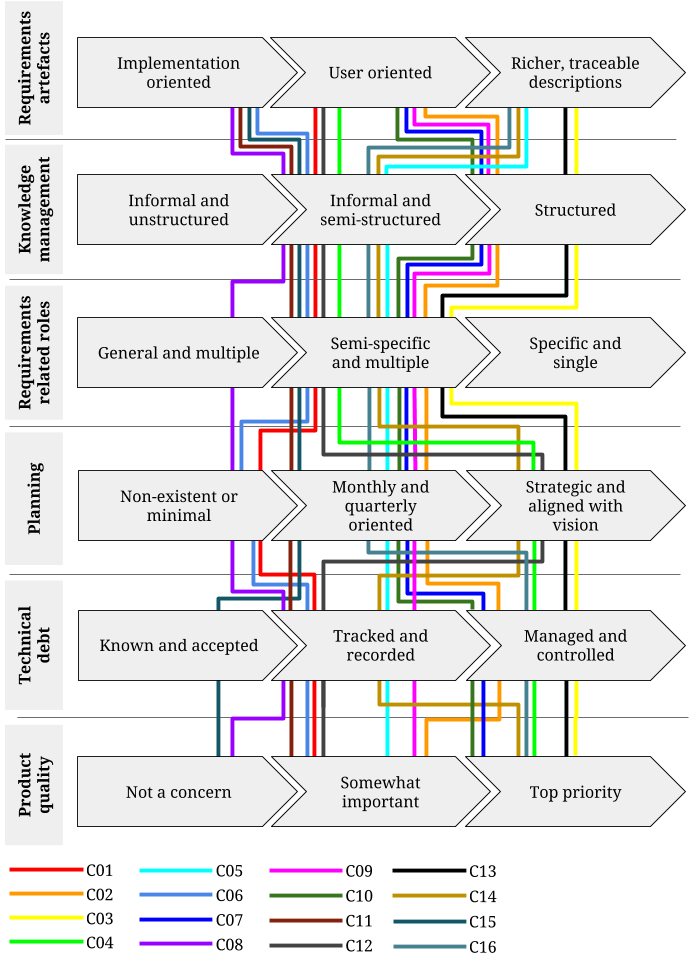
\psfig{file=companies-dimensions.png,width =3.4in}
\caption{Companies' Phases of Evolution}
\label{fig:companiesEvolution}
\end{figure}

\subsection{Discussion and Conclusions}
\label{sec:discussion}
Startups generally perceive requirements practices as a waste of time. In a fast-paced and reactive environment, they ignore the long run in order to capture a market, retain clients, and release products quicker. Evolution along the six dimensions are not fundamental to success. Factors that cause startups to die can be a combination of the market of its product, human resources, culture, funding, processes, and practices.

Figure \ref{fig:companiesEvolution} shows which phase of evolution of the six dimensions that each of the 16 companies are currently at. No startup reached the third phase of requirements-related roles and all had left the first phase of knowledge management. Company C06, a 10 year-old startup is only at phase one or two in every dimension.  It was reported that the work environment at C06 was stressful and had long hours. C03, one of the furthest along every dimension, was a 4 year-old startup with 11-20 employees. These contrasting profiles indicate that movement along the three phases of evolution is not dependent on company age and size. 



\section{Conclusions}
\label{sec:conclusions}

\section*{Acknowledgments}
\label{sec:acknowledgments}

Thanks Elena and Nic!

% The following two commands are all you need in the
% initial runs of your .tex file to
% produce the bibliography for the citations in your paper.
\bibliographystyle{abbrv}
% sample_paper.bib is the name of the BibTex file containing the
% bibliography entries. Note that you *don't* include the .bib ending here.
\bibliography{sample_paper}  
% You must have a proper ".bib" file
%  and remember to run:
% latex bibtex latex latex
% to resolve all references

\end{document}
